\documentclass[twocolumn,a4paper]{igs}
%\documentclass[review,letterpaper]{igs}

\usepackage{lineno}

\usepackage{verbatim,xspace,amsmath,amssymb}

\usepackage{tikz}
\usetikzlibrary{arrows}

\usepackage{igsnatbib}  % see igs2eguide.tex for example citation styles

\newcommand{\onecol}[1]{\includegraphics[width=86mm]{#1}}
\newcommand{\twocol}[1]{\includegraphics[width=178mm]{#1}}

% math macros
\newcommand\bb{\mathbf{b}}
\newcommand\bc{\mathbf{c}}
\newcommand\bbf{\mathbf{f}}
\newcommand\bn{\mathbf{n}}
\newcommand\bq{\mathbf{q}}
\newcommand\bu{\mathbf{u}}
\newcommand\bv{\mathbf{v}}
\newcommand\by{\mathbf{y}}

\newcommand\bF{\mathbf{F}}
\newcommand\bH{\mathbf{H}}
\newcommand\bQ{\mathbf{Q}}
\newcommand\bV{\mathbf{V}}
\newcommand\bW{\mathbf{W}}
\newcommand\bX{\mathbf{X}}

\newcommand\CC{\mathbb{C}}
\newcommand{\DDt}[1]{\ensuremath{\frac{d #1}{d t}}}
\newcommand{\ddt}[1]{\ensuremath{\frac{\partial #1}{\partial t}}}
\newcommand{\ddx}[1]{\ensuremath{\frac{\partial #1}{\partial x}}}
\newcommand{\ddy}[1]{\ensuremath{\frac{\partial #1}{\partial y}}}
\newcommand{\ddxp}[1]{\ensuremath{\frac{\partial #1}{\partial x'}}}
\newcommand{\ddz}[1]{\ensuremath{\frac{\partial #1}{\partial z}}}
\newcommand{\ddxx}[1]{\ensuremath{\frac{\partial^2 #1}{\partial x^2}}}
\newcommand{\ddyy}[1]{\ensuremath{\frac{\partial^2 #1}{\partial y^2}}}
\newcommand{\ddxy}[1]{\ensuremath{\frac{\partial^2 #1}{\partial x \partial y}}}
\newcommand{\ddzz}[1]{\ensuremath{\frac{\partial^2 #1}{\partial z^2}}}
\newcommand{\Div}{\nabla\cdot}
\newcommand\eps{\epsilon}
\newcommand{\grad}{\nabla}
\newcommand{\ihat}{\mathbf{i}}
\newcommand{\ip}[2]{\ensuremath{\left<#1,#2\right>}}
\newcommand{\jhat}{\mathbf{j}}
\newcommand{\khat}{\mathbf{k}}
\newcommand{\nhat}{\mathbf{n}}
\newcommand\lam{\lambda}
\newcommand\lap{\triangle}
\newcommand\RR{\mathbb{R}}
\newcommand\vf{\varphi}

\newcommand{\Mstar}{$\text{M}^{\bigstar}$\xspace}
\newcommand{\Mstarnoup}{$\text{M}^{\bigstar}_{\text{no}}$\xspace}
\newcommand{\Mstarfullup}{$\text{M}^{\bigstar}_{\text{full}}$\xspace}

\newcommand\alpharight{\alpha_{{}_{\blacktriangleright}}}
\newcommand\alphaup{\alpha_{{\!}_{\blacktriangle}}}

\newcommand{\dxtwo}{\tfrac{\Delta x}{2}}
\newcommand{\dytwo}{\tfrac{\Delta y}{2}}

\newcommand{\half}{\tfrac{1}{2}}


% fix lineno + amsmath bug
\newcommand*\patchAmsMathEnvironmentForLineno[1]{%
  \expandafter\let\csname old#1\expandafter\endcsname\csname #1\endcsname
  \expandafter\let\csname oldend#1\expandafter\endcsname\csname end#1\endcsname
  \renewenvironment{#1}%
     {\linenomath\csname old#1\endcsname}%
     {\csname oldend#1\endcsname\endlinenomath}}%
\newcommand*\patchBothAmsMathEnvironmentsForLineno[1]{%
  \patchAmsMathEnvironmentForLineno{#1}%
  \patchAmsMathEnvironmentForLineno{#1*}}%
\AtBeginDocument{%
\patchBothAmsMathEnvironmentsForLineno{equation}%
\patchBothAmsMathEnvironmentsForLineno{align}%
\patchBothAmsMathEnvironmentsForLineno{flalign}%
\patchBothAmsMathEnvironmentsForLineno{alignat}%
\patchBothAmsMathEnvironmentsForLineno{gather}%
\patchBothAmsMathEnvironmentsForLineno{multline}%
}


\begin{document}

\title[Stable schemes for the shallow ice approximation]{Stable finite volume element schemes \\ for the shallow ice approximation}

\abstract{The isothermal, non-sliding shallow ice approximation, combined with mass conservation, is a fundamental model for ice sheet and glacier flow.  It determines the ice geometry and extent by the solution of a free-boundary problem.  We solve the steady state form of this problem directly, without time-stepping, thereby demonstrating a fully-implicit scheme with no stability restrictions.  We first re-interpret the \cite{Mahaffy1976} finite difference method as a ``finite volume element'' scheme which has both an everywhere-defined approximate thickness function and a flux integral form of the conservation equation.  From this re-interpretation we build an improved scheme with better quadrature in the integral and upwinding on that part of the flux which is proportional to the bed gradient.  The discrete equations are then solved by a parallel Newton scheme which respects the constraint that ice thickness is nonnegative.  The results show better accuracy than published results on both flat bed and bedrock-step exact solutions.  We then apply the method at high resolution to model the steady-state geometry of the Greenland ice sheet, using only bedrock elevation and present-day surface mass balance as input data.}

\author{Ed Bueler}

\affiliation{Department of Mathematics and Statistics and Geophysical Institute, University of Alaska Fairbanks, USA \\
E-mail: \emph{\texttt{elbueler\@@alaska.edu}}}

\maketitle

\sectionsize


\section{Introduction}

The first successful numerical approach to modeling ice sheet flow and geometry evolution in two horizontal dimensions was the classical finite difference (FD) scheme introduced by \cite{Mahaffy1976}.  This scheme numerically solves the shallow ice approximation (SIA; Hutter, 1983)\nocite{Hutter1983} by computing the ice flux at staggered-grid points using particular choices when evaluating the ice thickness and surface slope.  An advantage of the scheme is its relatively-small stencil, which reduces memory usage in implicit or semi-implicit implementations \citep{HindmarshPayne1996} and interprocess communication in parallel implementations.

However, existing numerical models solve the time-dependent SIA using explicit or semi-implicit time-stepping  \citep{HindmarshPayne1996,Huybrechtsetal1996,Bueleretal2005,EgholmNielsen2010,JaroschSchoofAnslow2013}.  Time-stepping restrictions which arise in that context are needed to avoid classical instabilities at wavelengths comparable to the grid spacing \citep{MortonMayers2005}.  However, \cite{Bueleretal2005} and \cite{JaroschSchoofAnslow2013} point out that these schemes also involve \emph{ad hoc} treatment of the free margin of the ice sheet, for example using projection to reset computed negative thicknesses back to zero.  It would be desirable to escape both time-stepping restrictions and \emph{ad hoc} margins by implicitly solving the SIA free boundary problem in a mathematically-principled manner.

Early work on the free-boundary problem in one horizontal dimension \citep{Hindmarshetal1987} avoided \emph{ad hoc} margin treatment by tracking it as a moving grid point.  Such margin-tracking does not easily extend to two dimensions, however, because the margin of real ice sheets is an essentially-fractal curve of minimal smoothness and unknown-in-advance topology.  Calvo and others (2000; 2002)\nocite{CalvoDuranyVazquez2000,Calvoetal2002} avoid \emph{ad hoc} margins by describing the time-dependent problem as a parabolic complementarity problem which includes the constraint that ice thickness is never negative, but their work is also limited to one horizontal dimension and flat bed.  They solve each time step numerically by a projected Gauss-Siedel scheme \citep{Ciarlet2002}, which does not scale to large problem sizes.

\cite{JouvetBueler2012} pose and numerically-solve the steady-state free boundary problem as a variational inequality \citep{KinderlehrerStampacchia1980} in two spatial dimensions and with nontrivial bed topography.  Because this variational inequality is not equivalent to a minimization problem, in the general (non-flat-bed) case, they solve it by iterating well-posed, but only approximate, minimization problems which converge to the full equations in a fixed-point limit.  The success of this method is demonstrated in a 5 km grid steady-state calculation for Greenland using a piecewise-linear triangulation finite element (FE) method \citep{Elmanetal2005}.  In related work, \cite{JouvetGraeser2013} solve the SIA component of their time-stepping hybrid ice dynamics model \citep{Winkelmannetal2011} through a sequence of minimization problems which fix the thickness from the previous time-step.  Each minimization problem is solved by a constraint-adapted nonlinear multigrid Newton iteration.

In this paper we follow \cite{JouvetBueler2012} by solving the steady-state free boundary problem, but we use a Mahaffy-like scheme on a structured rectangular mesh and we apply the Newton iteration directly to the SIA problem.  A continuation scheme generates an iterate within the domain of convergence of the Newton method, which then exhibits quadratic convergence to the solution of the full SIA problem.  Our parallel implementation uses complementarity-problem Newton solvers \citep{BensonMunson2006} from the open-source PETSc library \citep{Balayetal2014}.  Because we successfully solve the whole free-boundary problem at once, our improved scheme is unconditionally stable as a fully-implicit scheme, at least when the bed is not too rough.

The first part of the paper has a historical side.  We re-interpret the classical Mahaffy scheme as using a non-standard quadrature choice in the conservation-of-mass flux integral.  In this re-interpretation the ice flux is everywhere-defined because the approximate ice thickness lives in a continuous space of trial functions, unlike in the original FD form of the scheme.  These trial functions are piecewise-bilinear on a structured grid of rectangles, that is, they are $Q^1$ finite elements \citep{Elmanetal2005}.  Because our re-interpretation has both finite volume \citep[FV;][]{LeVeque2002} and FE aspects, it is natural to regard the scheme as a ``finite volume element'' method \citep[FVE;][]{Cai1990,EwingLinLin2002} in which the weak form is simply the flux integral itself.  Adopting FVE terminology gives the best of both worlds: the unknown thickness is an everywhere-defined FE trial function and the discrete mass conservation equation is a flux-integral over a control volume (a la FV).

The paper is organized as follows.  We start with a statement of the steady, isothermal SIA model.  We then recall the classical Mahaffy scheme in FD form before re-interpreting it as an FVE scheme.  We then propose better quadrature in the flux integral, and we add a bit of first-order upwinding on the part of the flux that comes from the bedrock slope.  The resulting improved scheme, which has the same stencil as the classical Mahaffy scheme, is called ``\Mstar.''  Next we describe the Newton solver for the discrete equations and constraints, formulated as a nonlinear complementarity problem.  First numerical results in verification cases are excellent for a flat-bed dome exact solution and at least as good as those from higher-resolution upwind schemes on a bedrock-step exact solution.  Then we show how the method is applied to real ice sheets by computing the steady state shape of the Greenland ice sheet, in a present-day modeled climate, at high resolution including grids down to 600 m.  An Appendix addresses the analytical calculation of the Jacobian in the \Mstar scheme.


\section{Continuum model}

The time-dependent evolution equation for the ice thickness $H$ is a statement of mass conservation:
\begin{equation}
\frac{\partial H}{\partial t} + \Div \bq = m.  \label{eq:siaevolution}
\end{equation}
Here $\bq$ denotes the vertically-integrated flux and $m$ is the surface mass balance, also called the accumulation/ablation function.

The shallow ice approximation (SIA), the simplest relationship between $H$ and $\bq$ in common use in glaciology, is a lubrication approximation \citep{Fowler1997} of the Stokes equations for ice in non-sliding contact with the bed.  We only consider the isothermal, Glen-law \citep{GreveBlatter2009} case.  Let $b$ be the bed elevation and $s = H+b$ the ice surface elevation.  The flux $\bq$ is given by
\begin{equation}
\bq = - \Gamma H^{n+2} |\grad s|^{n-1} \grad s  \label{eq:siaflux}
\end{equation}
where $\Gamma = 2 A (\rho g)^n / (n+2)$ is a positive constant derived from the power $n\ge 1$, ice softness $A$, ice density $\rho$, and gravity $g$.

The flux $\bq$ has several forms equivalent to \eqref{eq:siaflux}.  For instance, because it is common to combine equations \eqref{eq:siaevolution} and \eqref{eq:siaflux} into a nonlinear diffusion equation \citep{Huybrechtsetal1996}, one may write
\begin{equation}
\bq = - D \grad s \quad \text{where} \quad D =  \Gamma H^{n+2} |\grad s|^{n-1}. \label{eq:siafluxdiffusion}
\end{equation}
Diffusion interpretation \eqref{eq:siafluxdiffusion} is appropriate in the flat-bed case because \eqref{eq:siaevolution} and \eqref{eq:siaflux} can be transformed to a $p$-Laplacian diffusion equation \citep{Calvoetal2002}, but a diffusion interpretation is obscured by the bed gradient $\grad b$.

If the bed is not flat then $\grad s$ and $\grad H$ are different, so the flux $\bq$ is not strictly diffusive because it is not opposite to the gradient of the conserved quantity, namely $H$.  For this reason, non-flat beds are also a barrier to proving well-posedness of the steady SIA  \citep{JouvetBueler2012}.

As an alternative to the diffusion form one can instead compute a vertically-averaged velocity $\bV$, and then treat the flux as arising from the transport of $H$ by $\bV$:
\begin{equation}
\bq = \bV H \quad \text{where} \quad \bV = - \Gamma H^{n+1} |\grad s|^{n-1} \grad s. \label{eq:siafluxvelocity}
\end{equation}
In this case \eqref{eq:siaevolution} is apparently a hyperbolic conservation equation, but this appearance is also deceiving because the velocity depends in part on the gradient of the transported quantity. 

Furthermore, nonzero $\grad b$ generates numerical conservation errors at the ice margin.  In addressing such errors \cite{JaroschSchoofAnslow2013} propose a third form for the flux, namely
\begin{equation}
   \bq = \boldsymbol{\omega} H^{n+2} \quad \text{where} \quad \boldsymbol{\omega} = - \Gamma |\grad s|^{n-1} \grad s. \label{eq:siafluxjsa}
\end{equation}
The vector field $\boldsymbol{\omega}$ can be thought of as a ``velocity'' which transports $H^{n+2}$.  In this thinking the combination of \eqref{eq:siaevolution} and \eqref{eq:siafluxjsa} becomes a kind of nonlinear hyperbolic equation, but again $\boldsymbol{\omega}$ depends on the gradient of the transported quantity $H$ so the combined equation is not truly hyperbolic.

We modify forms \eqref{eq:siafluxdiffusion} and \eqref{eq:siafluxjsa} to a split form
\begin{equation}
\bq = - D \grad H + \bW H^{n+2},\label{eq:fluxform}
\end{equation}
where $D$ is the same as in \eqref{eq:siafluxdiffusion} and where
\begin{equation}
\bW = - \Gamma |\grad s|^{n-1} \grad b.  \label{eq:siaWdefine}
\end{equation}
The vector field $\bW$ transports $H^{n+2}$, and in this case it is proportional to $\grad b$.  Only the magnitude of $\bW$ is influenced by $\grad H$.  Note that $\bW=0$ in the case of flat beds, while $\boldsymbol{\omega}$ is nonzero and $\bq$ is actually diffusive in that case.

In summary, the combination of \eqref{eq:siaevolution} with any of the above flux forms \eqref{eq:siaflux}--\eqref{eq:fluxform} defines a highly-nonlinear diffusion-advection equation.  Form \eqref{eq:fluxform} has the numerical advantage that we can apply a non-oscillatory transport scheme to $\bW H^{n+2}$ while also preserving accuracy by applying a centered scheme to $-D \grad H$.  The presence of the often-dominant leading-order diffusion is a motivation to use implicit time-stepping, not a common approach for hyperbolic problems.  Of course, implicit schemes for \eqref{eq:siaevolution} need to determine the location of the free boundary at each time step.

In this paper we will primarily solve the steady-state form of \eqref{eq:siaevolution}, namely
\begin{equation}
\Div \bq = m.  \label{eq:siasteady}
\end{equation}
By the divergence theorem, applied to any subregion $V$ of $\Omega$, we get the flux-integral form of the steady-state SIA, equivalent to \eqref{eq:siasteady},
\begin{equation}
  \int_{\partial V} \bq \cdot \bn\,ds = \int_V m\, dx\,dy. \label{eq:siaasconservation}
\end{equation}
Here $\partial V$ denotes the boundary of $V$, $\bn$ is the outward normal unit vector, and $ds$ is the length element on the closed curve $\partial V$.  Our numerical schemes will be based on \eqref{eq:siaasconservation}.

Equations \eqref{eq:siasteady} and \eqref{eq:siaasconservation} represent a boundary-value problem in which the location where the boundary conditions $H=0$ and $\bq=0$ apply is unknown \citep{JouvetBueler2012,JaroschSchoofAnslow2013}.  The ice-covered domain where \eqref{eq:siasteady} applies cannot be treated as a small modification of a known boundary, though that is the approach taken in explicit time-stepping schemes for equation \eqref{eq:siaevolution} \citep{Huybrechtsetal1996,Bueleretal2005}.

To be more precise about boundary conditions, if the surface mass balance $m$ is sufficiently-negative near the boundary of the computational domain $\Omega$ on which \eqref{eq:siasteady} is solved then $H\to 0$ at locations inside $\Omega$, namely at the ice margin or free boundary, at which $\bq \to 0$ simultaneously \citep{JouvetBueler2012}.  Because of the factor $H^{n+2}$ in formula \eqref{eq:siafluxdiffusion} for the diffusivity $D$, the problem has degenerate diffusivity, i.e.~also $D \to 0$ at the free boundary.  Solving equation \eqref{eq:siasteady}, or computing a time-step of \eqref{eq:siaevolution}, as such a free-boundary problem, without a boundary flux applied along any part of the boundary of $\Omega$, is usually called a ``whole'' ice sheet model.  We restrict our attention to such whole ice sheet models.

Thus we solve coupled equations \eqref{eq:siafluxdiffusion}, \eqref{eq:fluxform}, \eqref{eq:siaWdefine}, and \eqref{eq:siaasconservation}.  The input data consist of the bed elevation $b(x,y)$ and the (steady) surface mass balance $m(x,y)$.  These input data must be defined on a larger domain $\Omega$ than the ice-covered set.  We assume $m$ is sufficiently-negative near the boundary of $\Omega$ so that the ice-covered set is surrounded by ice-free areas.  Any contact with the ocean must be modeled as strongly negative values of $m$, and there is no modeled floating ice.  The solution is the nonnegative thickness function $H(x,y)$, defined everywhere in $\Omega$ and equal to zero where there is no ice.


\section{Methods}

\subsection{Classical Mahaffy scheme}

\begin{figure}[ht]
\begin{center}
\begin{tikzpicture}[scale=0.75]
  %uncomment to see grid on which it was generated:
  %\draw[dotted,step=1.0,black,very thin] (0,0) grid (6,4);

  % faint grid
  \draw[gray, dashed] (-0.75,0) -- (6.75,0);
  \draw[gray, dashed] (-0.75,2) -- (6.75,2);
  \draw[gray, dashed] (-0.75,4) -- (6.75,4);
  \draw[gray, dashed] (0,-0.5) -- (0,4.5);
  \draw[gray, dashed] (3,-0.5) -- (3,4.5);
  \draw[gray, dashed] (6,-0.5) -- (6,4.5);

  % regular FD points
  \filldraw (0,0) circle (2.5pt);
  \filldraw (3,0) circle (2.5pt);
  \filldraw (6,0) circle (2.5pt);
  \filldraw (0,2) circle (2.5pt);
  \filldraw (3,2) circle (2.5pt);
  \filldraw (6,2) circle (2.5pt);
  \filldraw (0,4) circle (2.5pt);
  \filldraw (3,4) circle (2.5pt);
  \filldraw (6,4) circle (2.5pt);

  % staggered FD points
  \def\dx{0.12};
  \filldraw (1.5-\dx,2+\dx) -- (1.5+\dx,2) -- (1.5-\dx,2-\dx) -- cycle;
  \filldraw (4.5-\dx,2+\dx) -- (4.5+\dx,2) -- (4.5-\dx,2-\dx) -- cycle;
  \filldraw (3-\dx,1-\dx) -- (3,1+\dx) -- (3+\dx,1-\dx) -- cycle;
  \filldraw (3-\dx,3-\dx) -- (3,3+\dx) -- (3+\dx,3-\dx) -- cycle;

  % dimensions \Delta x, \Delta y
  \draw[latex-latex] (3.2,4.5) -- (5.8,4.5);
  \draw (4.5,5.0) node {$\Delta x$};
  \draw[latex-latex] (6.5,2.2) -- (6.5,3.8);
  \draw (7.0,3) node {$\Delta y$};

  % label center point and dims
  \draw (3,-1.0) node {$x_j$};
  \draw (-1.25,2) node {$y_k$};

  % label as "a"
  \draw (-1.5,5.5) node {{\large a.}};
\end{tikzpicture}
 \quad 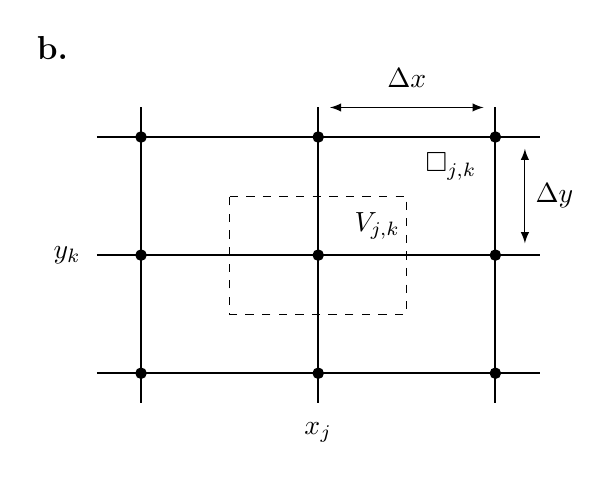
\begin{tikzpicture}[scale=0.75]
  %uncomment to see grid on which it was generated:
  %\draw[dotted,step=1.0,black,very thin] (0,0) grid (6,4);

  % strong grid around elements
  \draw[thick] (-0.75,0) -- (6.75,0);
  \draw[thick] (-0.75,2) -- (6.75,2);
  \draw[thick] (-0.75,4) -- (6.75,4);
  \draw[thick] (0,-0.5) -- (0,4.5);
  \draw[thick] (3,-0.5) -- (3,4.5);
  \draw[thick] (6,-0.5) -- (6,4.5);

  % nodes
  \filldraw (0,0) circle (2.5pt);
  \filldraw (3,0) circle (2.5pt);
  \filldraw (6,0) circle (2.5pt);
  \filldraw (0,2) circle (2.5pt);
  \filldraw (3,2) circle (2.5pt);
  \filldraw (6,2) circle (2.5pt);
  \filldraw (0,4) circle (2.5pt);
  \filldraw (3,4) circle (2.5pt);
  \filldraw (6,4) circle (2.5pt);

  % outline control volume
  \draw[dashed] (1.5,3) -- (4.5,3) -- (4.5,1) -- (1.5,1) -- cycle;

  % label element and control volume
  \draw (5.25,3.5) node {$\square_{j,k}$};
  \draw (4,2.5) node {$V_{j,k}$};

  % dimensions \Delta x, \Delta y
  \draw[latex-latex] (3.2,4.5) -- (5.8,4.5);
  \draw (4.5,5.0) node {$\Delta x$};
  \draw[latex-latex] (6.5,2.2) -- (6.5,3.8);
  \draw (7.0,3) node {$\Delta y$};

  % label center point and dims
  \draw (3,-1.0) node {$x_j$};
  \draw (-1.25,2) node {$y_k$};

  % label as "b"
  \tikzstyle{fontbf} = [font=\bf]
  \draw (-1.5,5.5) node[fontbf] {{\large b.}};
\end{tikzpicture}

\end{center}
\caption{\textbf{a.}~A structured FD grid with regular (dots) and staggered (triangles) points.  \textbf{b.}~The same grid as an FVE grid with rectangular elements $\square_{j,k}$ (solid), nodes (dots), a dual rectangular control volume $V_{j,k}$ (dashed), and Mahaffy's flux-evaluation locations (circles).  The corners of element $\square_{j,k}$ are indexed by $\ell$.}
\label{fig:fdfemgrids}
\end{figure}

Consider the rectangular structured FD grid, with spacing $\Delta x,\Delta y$, shown in Figure \ref{fig:fdfemgrids}a.  The \cite{Mahaffy1976} scheme calculates a flux component at each of the staggered grid points (triangles) based on values of other fields at regular points (dots).  For the staggered grid we introduce notation
\begin{equation}
x_j^\pm = x_j \pm \dxtwo, \qquad y_k^\pm = y_k \pm \dytwo. \label{eq:definexypm}
\end{equation}
At $(x_j^+,y_k)$ the scheme computes the $x$-component of the flux by
\begin{equation}
q^x_{j+\half,k} = - \Gamma (\hat H_{j+\half,k})^{\,n+2} \alpharight^{\,n-1} \frac{s_{j+1,k} - s_{j,k}}{\Delta x}  \label{eq:mahaffyqx}
\end{equation}
where $s_{j,k} = H_{j,k} + b_{j,k}$,
\begin{equation}
  \hat H_{j+\half,k} = \frac{H_{j,k} + H_{j+1,k}}{2},  \label{eq:mahaffyHav}
\end{equation}
and ``$\alpharight$\!'' is an estimate of $|\grad s|$:
\begin{align}
\alpharight^{\,2} &= \left(\frac{s_{j+1,k} - s_{j,k}}{\Delta x}\right)^2  \label{eq:mahaffyalphax} \\
  &\quad + \left(\frac{s_{j,k+1} + s_{j+1,k+1} - s_{j,k-1} - s_{j+1,k-1}}{4 \Delta y}\right)^2. \notag
\end{align}
At $(x_j,y_k^+)$ the scheme computes
\begin{equation}
q^y_{j,k+\half} = - \Gamma (\hat H_{j,k+\half})^{\,n+2} \alphaup^{\,n-1} \frac{s_{j,k+1} - s_{j,k}}{\Delta y}  \label{eq:mahaffyqy}
\end{equation}
where $\hat H_{j,k+\half}$ and $\alphaup$ are defined by swapping the roles of $j$ and $k$, and $\Delta x$ and $\Delta y$, in equations \eqref{eq:mahaffyHav} and \eqref{eq:mahaffyalphax}.  The slope approximation in \eqref{eq:mahaffyalphax} is perhaps the least-obvious aspect of the Mahaffy scheme, but one may check that these FD formulas are consistent \citep{MortonMayers2005} with \eqref{eq:siaflux}.

The discretization of mass conservation equation \eqref{eq:siasteady} itself uses straightforward centered-differences \citep{MortonMayers2005}:
\begin{equation}
\frac{q^x_{j+1/2,k} - q^x_{j-1/2,k}}{\Delta x} + \frac{q^y_{j,k+1/2}- q^y_{j,k-1/2}}{\Delta y} = m_{j,k}.  \label{eq:siasteadyfd}
\end{equation}
Equation \eqref{eq:siasteadyfd}, which relates the nine unknown values of $H$ at the regular grid points in Figure \ref{fig:fdfemgrids}a, the ``stencil'' of the scheme, is combined with \eqref{eq:mahaffyqx} and \eqref{eq:mahaffyqy} to give an equation in an algebraic system.


\subsection{FVE re-interpretation}

The above description of the Mahaffy FD method is familiar to numerical ice sheet modelers, but we now re-derive the scheme from an FVE perspective.  Our re-interpretation uses the same structured grid, but the regular grid points are now nodes (degrees of freedom) for a continuous space of trial functions.  Any FE method supposes that an approximation $H^h$ of the solution lies in a finite-dimensional space of functions which are sufficiently well-behaved so that the approximate flux $\bq^h$ is defined almost-everywhere.  In an FV method integral equation \eqref{eq:siaasconservation} is required to hold for a finite set of control volumes $V$ which together tile $\Omega$, which generates a finite system of nonlinear algebraic equations.

In Figure \ref{fig:fdfemgrids}b, element $\square_{j,k}$ is the rectangle with lower-left corner at $(x_j,y_k)$.  When associated with bilinear functions this rectangle is a $Q^1$ finite element \citep{Elmanetal2005}.  A basis for bilinear functions on $\square_{j,k}$ is the set
\begin{equation}
\chi_\ell \left(\frac{x-x_j}{\Delta x},\frac{y-y_k}{\Delta y}\right), \label{eq:elementbasis}
\end{equation}
for $\ell=0,1,2,3$, where
\begin{align*}
\chi_0(\xi,\eta) &= \left(1-\xi\right) \left(1-\eta\right), & \chi_1(\xi,\eta) &= \xi \left(1-\eta\right), \\
\chi_2(\xi,\eta) &= \xi \eta, & \chi_3(\xi,\eta) &= \left(1-\xi\right) \eta.
\end{align*}
With this order, $\chi_\ell=1$ on element corners traversed in counter-clockwise order (Figure \ref{fig:fdfemgrids}b).  

Let $S_h$ be the trial space of functions which are continuous on the whole computational domain $\Omega$ and bilinear on each element $\square_{j,k}$.  Functions in $S_h$ have a gradient which is defined almost everywhere, but the gradient is discontinuous along the element edges (solid lines in Figure \ref{fig:fdfemgrids}b).  We write $\psi_{j,k}(x,y)$ for the unique function in $S_h$ so that $\psi_{j,k}(x_r,y_s) = \delta_{jr} \delta_{ks}$ (Figure \ref{fig:fembases}a); such functions form a basis of $S_h$.

\begin{figure}[ht]
\begin{center}
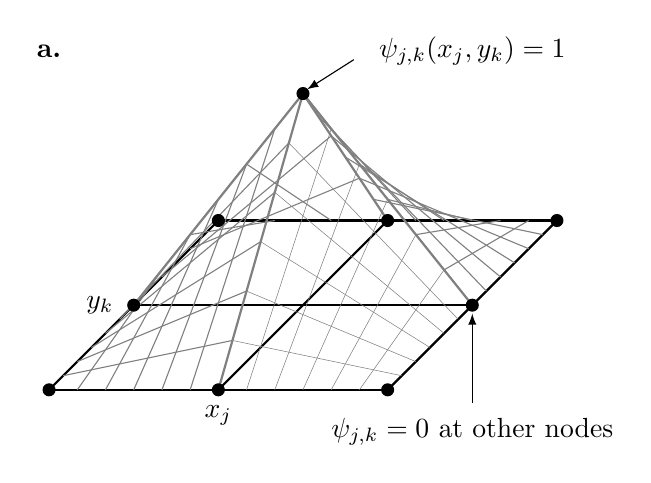
\begin{tikzpicture}[scale=8.6cm/16.0cm]
% min x = 0, max x = 12  so  width = 12 cm, but we pad
% 8.6cm is one-column width for J Glaciol
%\begin{tikzpicture}[scale=0.5]

  % strong grid around elements
  \draw[thick] (0,0) -- (8,0);
  \draw[thick] (2,2) -- (10,2);
  \draw[thick] (4,4) -- (12,4);
  \draw[thick] (0,0) -- (4,4);
  \draw[thick] (4,0) -- (8,4);
  \draw[thick] (8,0) -- (12,4);

  \def\ytop{7};

  % tent lines
  \draw[gray,thick] (6,\ytop) -- (4,0);
  \draw[gray,thick] (6,\ytop) -- (2,2);
  \draw[gray,thick] (6,\ytop) -- (10,2);
  \draw[gray,thick] (6,\ytop) -- (8,4);

  \def\dx{(10.0-6.0)/6};
  \def\dy{(2.0-\ytop)/6};
  \foreach \jj in {1,...,5}
  {
       \draw[gray,very thin] ({6+\jj*\dx},{\ytop+\jj*\dy}) -- ({4+(4/6)*\jj},0.0);
  }

  \def\dx{(4.0-6.0)/6};
  \def\dy{(0.0-\ytop)/6};
  \foreach \jj in {1,...,5}
  {
       \draw[gray,very thin] ({6+\jj*\dx},{\ytop+\jj*\dy}) -- ({10-(2/6)*\jj},{2-(2/6)*\jj});
  }

  \def\dx{(2.0-6.0)/6};
  \def\dy{(2.0-\ytop)/6};
  \foreach \jj in {1,...,5}
  {
       \draw[gray,thin] ({6+\jj*\dx},{\ytop+\jj*\dy}) -- ({4-(4/6)*\jj},0.0);
  }

  \def\dx{(4.0-6.0)/6};
  \def\dy{(0.0-\ytop)/6};
  \foreach \jj in {1,...,5}
  {
       \draw[gray,thin] ({6+\jj*\dx},{\ytop+\jj*\dy}) -- ({2-(2/6)*\jj},{2-(2/6)*\jj});
  }

  \def\dx{(10.0-6.0)/6};
  \def\dy{(2.0-\ytop)/6};
  \foreach \jj in {1,...,5}
  {
       \draw[gray,thin] ({6+\jj*\dx},{\ytop+\jj*\dy}) -- ({8+(4/6)*\jj},4.0);
  }

  \def\dx{(8.0-6.0)/6};
  \def\dy{(4.0-\ytop)/6};
  \foreach \jj in {1,...,5}
  {
       \draw[gray,thin] ({6+\jj*\dx},{\ytop+\jj*\dy}) -- ({10+(2/6)*\jj},{2+(2/6)*\jj});
  }

  \def\dx{(2.0-6.0)/3};
  \def\dy{(2.0-\ytop)/3};
  \foreach \jj in {1,...,2}  % reduce clutter
  {
       \draw[gray,thin] ({6+\jj*\dx},{\ytop+\jj*\dy}) -- ({8-(4/3)*\jj},4.0);
  }

  \def\dx{(8.0-6.0)/3};
  \def\dy{(4.0-\ytop)/3};
  \foreach \jj in {1,...,2}
  {
       \draw[gray,thin] ({6+\jj*\dx},{\ytop+\jj*\dy}) -- ({2+(2/3)*\jj},{2+(2/3)*\jj});
  }

  % nodes in base plane
  \filldraw (0,0) circle (4pt);
  \filldraw (4,0) circle (4pt);
  \filldraw (8,0) circle (4pt);
  \filldraw (2,2) circle (4pt);
  %\filldraw (6,2) circle (4pt);   % (x_j,y_k) is at (6,2)
  \filldraw (10,2) circle (4pt);
  \filldraw (4,4) circle (4pt);
  \filldraw (8,4) circle (4pt);
  \filldraw (12,4) circle (4pt);

  % node at tent top
  \filldraw (6,\ytop) circle (4pt);

  % annotate
  \draw (10,\ytop+1.0) node {$\psi_{j,k}(x_j,y_k)=1$};
  \draw[-latex] (7.2,\ytop+0.8) -- (6.1,\ytop+0.1);
  \draw (10,-1.0) node {$\psi_{j,k}=0$ at other nodes};
  \draw[-latex] (10,-0.3) -- (10,1.8);

  % label center point
  \draw (4,-0.6) node {$x_j$};
  \draw (1.2,2) node {$y_k$};

  % label as "a"
  \tikzstyle{fontbf} = [font=\bf]
  \draw (0,8) node[fontbf] {a.};

\end{tikzpicture}
 \quad 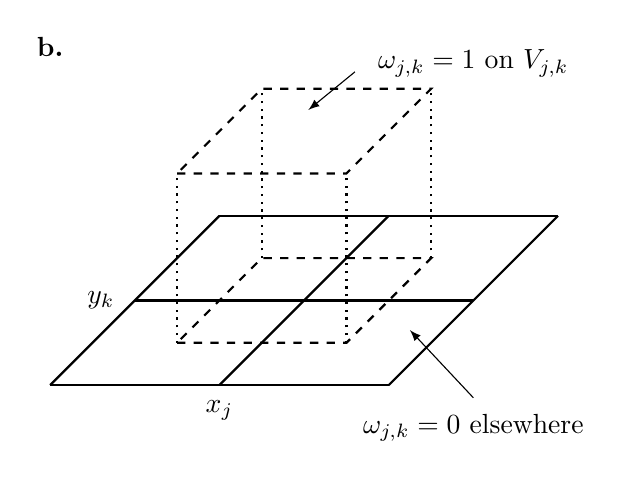
\begin{tikzpicture}[scale=8.6cm/16.0cm]
% min x = 0, max x = 12  so  width = 12 cm, but we pad
% 8.6cm is one-column width for J Glaciol
%\begin{tikzpicture}[scale=0.5]

  % strong grid around elements
  \draw[thick] (0,0) -- (8,0);
  \draw[thick] (2,2) -- (10,2);
  \draw[thick] (4,4) -- (12,4);
  \draw[thick] (0,0) -- (4,4);
  \draw[thick] (4,0) -- (8,4);
  \draw[thick] (8,0) -- (12,4);

  % dashed grid around control volume in base plane
  \draw[thick] (0,0) -- (8,0);

  % label element and control volume
  \def\lift{4};
  \draw[dashed, thick] (3,1) -- (7,1) -- (9,3) -- (5,3) -- cycle;
  \draw[dashed, thick] (3,1+\lift) -- (7,1+\lift) -- (9,3+\lift) -- (5,3+\lift) -- cycle;
  \draw[dotted, thick] (3,1) -- (3,1+\lift);
  \draw[dotted, thick] (7,1) -- (7,1+\lift);
  \draw[dotted, thick] (9,3) -- (9,3+\lift);
  \draw[dotted, thick] (5,3) -- (5,3+\lift);

  % annotate
  \draw (10,\lift+3.6) node {$\omega_{j,k}=1$ on $V_{j,k}$};
  \draw[-latex] (7.2,\lift+3.4) -- (6.1,\lift+2.5);
  \draw (10,-1.0) node {$\omega_{j,k}=0$ elsewhere};
  \draw[-latex] (10,-0.3) -- (8.5,1.3);

  % label center point
  \draw (4,-0.6) node {$x_j$};
  \draw (1.2,2) node {$y_k$};

  % label as "b"
  \tikzstyle{fontbf} = [font=\bf]
  \draw (0,8) node[fontbf] {b.};

\end{tikzpicture}

\end{center}
\caption{\textbf{a.}~A continuous ``hat'' basis function $\psi_{j,k}$ in the trial space $S_h$.  \textbf{b.}~A full FE interpretation would use piecewise-constant basis functions $\omega_{j,k}$ from the test space $S_h^*$.}
\label{fig:fembases}
\end{figure}

We seek an approximate solution $H^h$ from $S_h$.  Also let $b^h$ in $S_h$ be the interpolant of the bed elevation data $b$, and let $s^h=H^h+b^h$.  We denote by $\bq^h$ the flux computed from formula \eqref{eq:fluxform} using $H^h$, $b^h$, and $s^h$, so that $\bq^h$ is well-defined on the interior of each element.

Let $V_{j,k}$ be the control volume with center at $(x_j,y_k)$ shown in Figure \ref{fig:fdfemgrids}b.  In the FVE method we require \eqref{eq:siaasconservation} to hold for $\bq=\bq^h$ and $V$ equal to each $V_{j,k}$.  Because we use a periodic grid with $N_x$ rectangles in the $x$-direction and $N_y$ in the $y$-direction, there are $N=N_xN_y$ nodes, $N$ distinct control volumes, and $N$ equations in the algebraic system.

Instead of control volumes, in a full FE interpretation we would introduce test functions, as follows.  Let $S_h^*$ be the space of functions which are constant on each control volume $V_{j,k}$.  These functions are piecewise-constant and (generally) discontinuous only along the control volume edges.  Bases of both spaces $S_h$ and $S_h^*$ are formed by those functions which are one at a single node and zero at all other nodes; Figure \ref{fig:fembases}b shows such a function $\omega_{j,k}$.  Requiring \eqref{eq:siaasconservation} to hold for each control volume in our FVE method is equivalent to multiplying \eqref{eq:siasteady} by $\omega_{j,k}$ and then integrating-by-parts, but showing the equivalence requires generalized functions.  (The derivative of a step function is a Dirac delta function.)  We adopt the FVE interpretation, however, so we have no further need for test functions from $S_h^*$.

Both the classical Mahaffy scheme, and our improved scheme below, assume midpoint quadrature on the right-hand integral in \eqref{eq:siaasconservation}, so we seek $H^h$ in $S_h$ satisfying
\begin{equation}
  \int_{\partial V_{j,k}} \bq^h \cdot \bn\,ds = m_{j,k}\, \Delta x \Delta y \label{eq:siafve}
\end{equation}
for all $j,k$.  It remains to do quadrature on the left in \eqref{eq:siafve}, however.  We decompose the integral over the four edges of $\partial V_{j,k}$:
\begin{align}
\int_{\partial V_{j,k}} \bq^h \cdot \bn\,ds &= \int_{y_k^-}^{y_k^+} q^x(x_j^+,y)\,dy \label{eq:fluxintdecomp} \\
&\quad + \int_{x_j^-}^{x_j^+} q^y(x,y_k^+)\,dx \notag \\
&\quad - \int_{y_k^-}^{y_k^+} q^x(x_j^-,y)\,dy \notag \\
&\quad - \int_{x_j^-}^{x_j^+} q^y(x,y_k^-)\,dx. \notag
\end{align}
The flux $\bq^h$ is a bounded function which is discontinuous across element boundaries.  In the first right-hand integral in \eqref{eq:fluxintdecomp} the integrand $f(y) = q^x(x_j^+,y)$ has a jump discontinuity at the midpoint of the interval of integration (i.e.~at $y=y_k$).  Specifically, $\partial s^h/\partial y = s^h_y$ is discontinuous at $y=y_k$.  But formula \eqref{eq:mahaffyqx} in the Mahaffy FD scheme computes the normal component of $\bq^h$ exactly at that midpoint.

The key to re-interpreting the Mahaffy scheme is to see that it computes each integral in \eqref{eq:fluxintdecomp} by the midpoint method \emph{using averages of the discontinuous surface gradient across its jump discontinuities}.  The scheme does not use true quadrature because the integrand $\bq^h\cdot \bn$ does not have a value at the quadrature point.

To turn this idea into formulas, observe that both the thickness $H^h$ and the $x$-derivative $\partial s^h/\partial x = s^h_x$ are continuous along the edge between elements $\square_{j,k}$ and $\square_{j,k-1}$.  In fact, using the element basis \eqref{eq:elementbasis} the surface gradient on $\square_{j,k}$ has components
\begin{align}
s^h_x(x,y) &= \frac{s_{j+1,k}-s_{j,k}}{\Delta x} \left(1-\frac{y-y_k}{\Delta y}\right)  \label{eq:grads} \\
   &\quad + \frac{s_{j+1,k+1}-s_{j,k+1}}{\Delta x} \left(\frac{y-y_k}{\Delta y}\right), \notag \\
s^h_y(x,y) &= \frac{s_{j,k+1}-s_{j,k}}{\Delta y} \left(1-\frac{x-x_j}{\Delta x}\right) \notag \\
   &\quad + \frac{s_{j+1,k+1}-s_{j+1,k}}{\Delta y} \left(\frac{x-x_j}{\Delta x}\right). \notag
\end{align}
On $\square_{j,k-1}$, $s^h_x$ and $s^h_y$ can be calculated by shifting the index $k$ to $k-1$.  Thus the continuous function $s^h_x$ has value
\begin{equation}
s^h_x(x_j^+,y_k) = \frac{s_{j+1,k}-s_{j,k}}{\Delta x} \label{eq:femsxstag}
\end{equation}
at the midpoint $y=y_k$ in the first integral in \eqref{eq:fluxintdecomp}.  Similarly, writing-out $H^h$ using element basis \eqref{eq:elementbasis} gives
\begin{equation}
H^h(x_j^+,y_k) = \frac{H_{j,k}+H_{j+1,k}}{2} \label{eq:femHstag}
\end{equation}
at the midpoint, which is \eqref{eq:mahaffyHav}.  But the $y$-derivative $s^h_y$ has different values above (on $\square_{j,k}$) and below (on $\square_{j,k-1}$) the element boundary at $y = y_k$.  The limits are:
\begin{align}
s^h_y(x_j^+,y_k\!+\!0) = \frac{s_{j,k+1}-s_{j,k} + s_{j+1,k+1}-s_{j+1,k}}{2\Delta y}, \\
s^h_y(x_j^+,y_k\!-\!0) = \frac{s_{j,k}-s_{j,k-1} + s_{j+1,k}-s_{j+1,k-1}}{2\Delta y}. \notag
\end{align}
The average of these values is not a value of $s_y^h$, but a re-construction:
\begin{equation}
\widehat{s^h_y}(x_j^+,y_k) = \frac{s_{j,k+1} + s_{j+1,k+1} - s_{j,k-1} - s_{j+1,k-1}}{4\Delta y}. \label{eq:femsystagcrime}
\end{equation}
Formula \eqref{eq:femsystagcrime} is exactly the estimate of $\partial s/\partial y$ which appears in Mahaffy's FD formula \eqref{eq:mahaffyalphax}.

In our FVE re-interpretation, the Mahaffy scheme uses \eqref{eq:femsxstag}, \eqref{eq:femHstag}, and \eqref{eq:femsystagcrime} in the midpoint rule for the first integral in \eqref{eq:fluxintdecomp}
\begin{align}
&\int_{y_k^-}^{y_k^+} q^x(x_j^+,y)\,dy  \label{eq:femmahaffyfirstint} \\
  &\quad\approx - \Delta y\, \Gamma H^h(x_j^+,y_k)^{n+2} \,\alpharight^{\,(n-1)/2} s^h_x(x_j^+,y_k). \notag 
\end{align}
where
\begin{equation}
\alpharight^2 = s^h_x(x_j^+,y_k)^2 + \widehat{s^h_y}(x_j^+,y_k)^2
\end{equation}
is the same as in \eqref{eq:mahaffyalphax}.  Thus Mahaffy's scheme approximates each integral on the right in \eqref{eq:fluxintdecomp} by a perfectly-reasonable quadrature ``crime'' \citep[compare][]{Strang1972} which averages across a discontinuity to reconstruct a slope.  Recognizing the Mahaffy choice as quadrature-like, in this FVE context, is beneficial because it allows us to do it better.


\subsection{Improved scheme}

If the goal is to accurately-generate an algebraic equation from \eqref{eq:siafve} by quadrature along $\partial V_{j,k}$ then it is easy to improve upon the Mahaffy technique by improving quadrature.  We also use flux decomposition \eqref{eq:fluxform} with an upwind-type discretization on the bed gradient term $\bW H^{n+2}$.  Together these improvements define the ``\Mstar'' scheme.

As already noted, the numerical approximation $\bq^h$ from \eqref{eq:fluxform} is defined and smooth on the interior of each element, but discontinuous across element boundaries.  So we break each interval of integration on the right side of \eqref{eq:fluxintdecomp} into two parts and use the midpoint rule, the optimal one-point rule, on each half.  For example, we break the first integral at $y=y_k$:
\begin{align}
&\int_{y_k^-}^{y_k^+} q^x(x_j^+,y)\,dy  \label{eq:starbreakfirst} \\
  &\quad= \int_{y_k^-}^{y_k} q^x(x_j^+,y)\,dy + \int_{y_k}^{y_k^+} q^x(x_j^+,y)\,dy \notag \\
  &\quad\approx \frac{\Delta y}{2} \left(q^x(x_j^+,y_k-\tfrac{\Delta y}{4}) + q^x(x_j^+,y_k+\tfrac{\Delta y}{4})\right). \notag
\end{align}
Recalling notation \eqref{eq:definexypm}, values $q^x(x_j^+,y_k\pm\tfrac{\Delta y}{4})$ are evaluations of $\bq^h$ at points of continuity.  Similar formulas to \eqref{eq:starbreakfirst} apply to the other three integrals on the right side of \eqref{eq:fluxintdecomp}.

\begin{figure}[ht]
\begin{center}
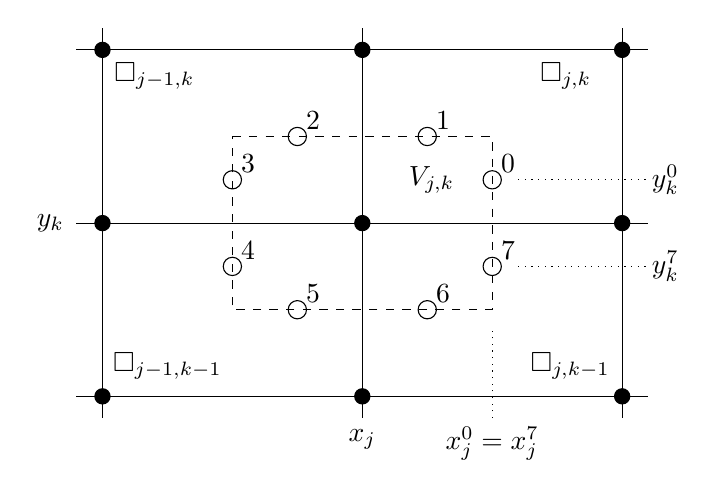
\begin{tikzpicture}[scale=1.1]
  %uncomment to see grid on which it was generated:
  %\draw[dotted,step=1.0,black,very thin] (0,0) grid (6,4);

  % strong grid around elements
  \draw (-0.3,0) -- (6.3,0);
  \draw (-0.3,2) -- (6.3,2);
  \draw (-0.3,4) -- (6.3,4);
  \draw (0,-0.25) -- (0,4.25);
  \draw (3,-0.25) -- (3,4.25);
  \draw (6,-0.25) -- (6,4.25);

  % nodes
  \filldraw (0,0) circle (2.5pt);
  \filldraw (3,0) circle (2.5pt);
  \filldraw (6,0) circle (2.5pt);
  \filldraw (0,2) circle (2.5pt);
  \filldraw (3,2) circle (2.5pt);
  \filldraw (6,2) circle (2.5pt);
  \filldraw (0,4) circle (2.5pt);
  \filldraw (3,4) circle (2.5pt);
  \filldraw (6,4) circle (2.5pt);

  % outline control volume
  \draw[dashed] (1.5,3) -- (4.5,3) -- (4.5,1) -- (1.5,1) -- cycle;

  % mark quadrature points

  \draw (4.5,2.5) circle (3.0pt) node[shift={(0.2,0.2)}] {0};
  \draw (3.75,3)  circle (3.0pt) node[shift={(0.2,0.2)}] {1};
  \draw (2.25,3)  circle (3.0pt) node[shift={(0.2,0.2)}] {2};
  \draw (1.5,2.5) circle (3.0pt) node[shift={(0.2,0.2)}] {3};
  \draw (1.5,1.5) circle (3.0pt) node[shift={(0.2,0.2)}] {4};
  \draw (2.25,1)  circle (3.0pt) node[shift={(0.2,0.2)}] {5};
  \draw (3.75,1)  circle (3.0pt) node[shift={(0.2,0.2)}] {6};
  \draw (4.5,1.5) circle (3.0pt) node[shift={(0.2,0.2)}] {7};

  % label elements and control volume
  \draw (3.8,2.5) node {$V_{j,k}$};
  \draw (5.35,3.7) node {$\square_{j,k}$};
  \draw (5.4,0.35) node {$\square_{j,k-1}$};
  \draw (0.6,3.7) node {$\square_{j-1,k}$};
  \draw (0.75,0.35) node {$\square_{j-1,k-1}$};

  % label center point
  \draw (3,-0.5) node {$x_j$};
  \draw (-0.6,2) node {$y_k$};

  % indicate coordinates of quadrature points
  \draw[dotted] (4.5,-0.25) -- (4.5, 0.8);
  \draw (4.5,-0.55) node {$x_j^0=x_j^7$};
  \draw[dotted] (4.8,2.5) -- (6.3, 2.5);
  \draw (6.5,2.5) node {$y_k^0$};
  \draw[dotted] (4.8,1.5) -- (6.3, 1.5);
  \draw (6.5,1.5) node {$y_k^7$};

\end{tikzpicture}

\end{center}
\caption{For equation \eqref{eq:siamstar} we evaluate $\bq^h(x,y)$ at eight quadrature points (numbered circles) along $\partial V_{j,k}$ (dashed).}
\label{fig:improvequadrature}
\end{figure}

Figure \ref{fig:improvequadrature} shows all eight quadrature points needed to compute the full integral over $\partial V_{j,k}$ in \eqref{eq:siafve}.  At each quadrature point we evaluate the $x$- or $y$-component of $\bq^h$ and multiply by a constant to get the appropriate integral.  Our approximation of \eqref{eq:siafve} is
\begin{equation}
\sum_{s=0}^7 \bc_s \cdot \bq^h(x_j^s,y_k^s) = m_{j,k}\,\Delta x\,\Delta y  \label{eq:siamstar}
\end{equation}
where
\begin{align}
\bc_0 &= \bc_7 = \left(0, \tfrac{\Delta y}{2}\right),  \label{eq:cs} \\
\bc_1 &= \bc_2 = \left(\tfrac{\Delta x}{2},0\right),  \notag \\
\bc_3 &= \bc_4 = \left(0, -\tfrac{\Delta y}{2}\right),  \notag \\
\bc_5 &= \bc_6 = \left(-\tfrac{\Delta x}{2},0\right),  \notag
\end{align}
and
\begin{align}
x_j^0 &= x_j^7 = x_j + \tfrac{\Delta x}{2}, & y_k^1 &= y_k^2 = y_k + \tfrac{\Delta y}{2}, \label{eq:xjsyks} \\
x_j^1 &= x_j^6 = x_j + \tfrac{\Delta x}{4}, & y_k^0 &= y_k^3 = y_k + \tfrac{\Delta y}{4}, \notag \\
x_j^2 &= x_j^5 = x_j - \tfrac{\Delta x}{4}, & y_k^4 &= y_k^7 = y_k - \tfrac{\Delta y}{4}, \notag \\
x_j^3 &= x_j^4 = x_j - \tfrac{\Delta x}{2}, & y_k^5 &= y_k^6 = y_k - \tfrac{\Delta y}{2}. \notag
\end{align}

Implementing equation \eqref{eq:siamstar} requires evaluating $\bq^h$ at eight quadrature points, twice the number for the classical method, but the stencils are the same because we use the same nine nodal values of $H^h$.  One could propose further-improved quadrature, replacing the midpoint rule by higher-order methods (e.g.~2-point Gauss-Legendre).  Also, our $Q^1$ elements could be replaced by higher-order (e.g.~$Q^2$) elements.  Though such methods have not been tested, in fact the largest numerical SIA errors occur near the ice margin where the solution $H$ has unbounded gradient \citep{Bueleretal2005}.  Thus higher-order quadrature and interpolation will not give much advantage.  We believe our improved method represents a measurable accuracy and Newton-iteration-convergence improvement over the classical Mahaffy method (Results section) because it evaluates $\bq^h$ at points of continuity, not because the order of quadrature or interpolation is flawed in the classical scheme.

\cite{JaroschSchoofAnslow2013} show that the Mahaffy scheme can suffer from significant mass conservation errors at locations of abrupt change in the bed elevation.  In such cases where the bed gradient dominates the flux, the mass conservation equation has ``hyperbolic'' character.  Thus they use a high-resolution upwind scheme \citep{LeVeque2002} based on flux form \eqref{eq:siafluxjsa}.  They show reduced mass conservation errors in the sense of giving numerical solutions which are closer in volume to an exact solution.  On the other hand, their scheme, which solves the time-dependent problem \eqref{eq:siaevolution} using explicit time-stepping, expands the stencil because it needs values two grid spaces away.

By comparison, we propose using minimal first-order upwinding based on form \eqref{eq:fluxform} of the flux, even though upwinding is not required for linear stability or non-oscillation of our implicit scheme \citep{MortonMayers2005}.  Numerical testing suggests upwinding is effective in our case because it improves the conditioning of the Jacobian matrix used in the Newton iteration (not shown).

In our improved scheme the transport flux $\tilde \bq = \bW H^{n+2}$ uses $H$ evaluated at a location different from the quadrature point, according to the direction of $\bW$ evaluated at the quadrature point.  For instance, our upwind modification at $(x_j^0,y_k^0)$---see Figure \ref{fig:improvequadrature}---uses the sign of
\begin{equation}
W^x_* = W^x(x_j^0,y_k^0),
\end{equation}
where $\bW=(W^x,W^y)$.  Note that the sign of $W_x^*$ is opposite that of the $x$-component of $\grad b^h$ at $(x_j^0,y_k^0)$.  We shift the evaluation of $H$ upwind by a fraction $0\le \lambda \le 1$ of an element width,
\begin{align}
&\tilde \bq^x(x_j^0,y_k^0)  \label{eq:upwindschemex} \\
&\quad = W^x_* \begin{cases}
                 H(x_j^0-\lambda \tfrac{\Delta x}{2},y_k^0)^{n+2}, & W^x_* \ge 0, \\
                 H(x_j^0+\lambda \tfrac{\Delta x}{2},y_k^0)^{n+2}, & W^x_* < 0,
             \end{cases} \notag
\end{align}
where $\lambda=0$ is no upwinding and $\lambda=1$ is the maximum upwinding that does not expand the stencil.  After experimentation (Results section) we chose $\lambda=1/4$ (Figure \ref{fig:upwindterm}).  This value is seen to be large enough to improve the convergence of the Newton iteration but also small enough to generate substantial improvements in accuracy for the bedrock-step exact solution.  Upwinding at the other seven points along $\partial V_{j,k}$ (Figure \ref{fig:improvequadrature}) uses similar formulas.

\begin{figure}[ht]
\begin{center}
\begin{tikzpicture}[scale=1.8]
  %uncomment to see grid on which it was generated:
  %\draw[dotted,step=1.0,black,very thin] (0,0) grid (6,4);

  % strong grid around elements
  \draw (-0.3,0) -- (3.3,0);
  \draw (-0.3,2) -- (3.3,2);
  \draw (0,-0.3) -- (0,2.3);
  \draw (3,-0.3) -- (3,2.3);

  % nodes
  \filldraw (0,0) circle (1.5pt);
  \filldraw (3,0) circle (1.5pt);
  \filldraw (0,2) circle (1.5pt);
  \filldraw (3,2) circle (1.5pt);

  % outline control volume
  \draw[dashed, thick] (-0.25,1) -- (1.5,1) -- (1.5,-0.25);

  % mark quadrature points
  \draw (1.5,0.5)  circle (2.0pt);
  \draw (0.75,1.0) circle (2.0pt);

  % mark upwind points
  \draw (1.125,0.5) node {$+$};
  \draw (1.875,0.5) node {$+$};
  \draw (0.75,0.75) node {$+$};
  \draw (0.75,1.25) node {$+$};

  % arrows to suggest upwinding
  %\draw[-latex] (1.6,0.4) -- (1.80,0.4);
  %\draw[-latex] (1.4,0.4) -- (1.20,0.4);
  %\draw[-latex] (0.65,1.05) -- (0.65,1.2);
  %\draw[-latex] (0.65,0.95) -- (0.65,0.8);

  % label elements and control volume
  \draw (2.7,1.7) node {$\square_{j,k}$};

  % label lower-left corner
  \draw (0,-0.5) node {$x_j$};
  \draw (-0.5,0) node {$y_k$};

  % indicate coordinates of quadrature point
  \draw (1.5,-0.5) node {$x_j^0$};
  \draw[dotted] (2.8,0.5) -- (3.2, 0.5);
  \draw (3.4,0.52) node {$y_k^0$};

\end{tikzpicture}

\end{center}
\caption{On element $\square_{j,k}$, when computing the flux at quadrature points (circles), upwinding of the flux term $\tilde \bq = \bW H^{n+2}$ evaluates the thicknesses $H$ at locations shown with ``$+$'', one quarter of the way to the element boundary.}
\label{fig:upwindterm}
\end{figure}

The ``\Mstar'' scheme combines both improvements, namely better quadrature and a bit of upwinding.  We will see in verification (Results section) that it achieves higher solution accuracy than either the apparently second-order Mahaffy scheme or the higher-resolution explicit advection scheme of \cite{JaroschSchoofAnslow2013}.  (As our Newton solver needs a differentiable residual function, the additional non-smoothness of high-resolution flux methods suggests caution.)  Convergence of the Newton iteration is also improved compared to the classical Mahaffy scheme.  The evidence suggests that our form of upwinding is most important at locations of low regularity of the solution.


\subsection{Solution of the equations}

We are ready to write down a system of nonlinear algebraic equations, but it remains to describe the numerical solution of this system.  This is nontrivial because inequality constraints apply to each unknown.

Each equation from the \Mstar scheme is simply \eqref{eq:siamstar} with an upwind modification like \eqref{eq:upwindschemex} at the quadrature points.  The resulting highly-nonlinear system of $N=N_x N_y$ equations is
\begin{equation}
F_{j,k}(\bH) = 0.   \label{eq:nonlinsystem}
\end{equation}
This determines $N$ unknowns, a vector $\bH=\{H_{j,k}\}$; note $H^h(x,y)$ and $\bH$ are actually two representations of the same discrete thickness approximation.  System \eqref{eq:nonlinsystem} is not adequate by itself, however, because each unknown thickness $H_{j,k}$ must be nonnegative, i.e.
\begin{equation}
\bH \ge 0.  \label{eq:nonlinconstraints}
\end{equation}

Requirements \eqref{eq:nonlinsystem} and \eqref{eq:nonlinconstraints} can be combined into a variational inequality \citep{JouvetBueler2012,KinderlehrerStampacchia1980}.  Equivalently, we can write them in complementarity problem form \citep{BensonMunson2006}:
\begin{equation}
\bH \ge 0, \quad \bF(\bH) \ge 0, \quad \bH \cdot \bF(\bH) = 0.  \label{eq:nonlincomplementarity}
\end{equation}
We will solve \eqref{eq:nonlincomplementarity} by a ``constrained'' Newton solver, specifically by either the reduced-space or semi-smooth methods \citep{BensonMunson2006} implemented in PETSc \citep{Balayetal2014}.  Our open-source C code\footnote{Clone the repository at \texttt{https://github.com/bueler/sia-fve}.  Then see \texttt{README.md} in directory \texttt{petsc/} to compile \texttt{mahaffy.c} and run the examples.} contains residual and Jacobian evaluation subroutines, but parallel grid management, Newton solver, iterative linear solver, and linear preconditioning are all consigned to PETSc choices made at runtime.  Both multigrid \citep{Briggsetal2000} and additive-Schwarz-type domain decomposition \citep{Smithetal1996} preconditioning are found to work, but the latter is more robust and is used in all runs in the Results section.

The Jacobian of system \eqref{eq:nonlinsystem}, i.e.~the $N\times N$ matrix
\begin{equation}
J = \left(\,\frac{\partial F_{j,k}}{\partial H_{p,q}}\,\right), \label{eq:nonlinjacobian}
\end{equation}
can be computed via hand-calculated derivatives.  This additional effort (Appendix) gives a speed-up by a rough factor of 1.5 over the alternative, namely finite-difference (FD) computation of Jacobian entries coming from additional residual (i.e.~$F$) evaluations.  Such FD Jacobians are efficiently-implemented in PETSc using ``coloring'' of the nodes \citep{CurtisPowellReid1974} so that, from the nine-point stencil, only ten residual evaluations are needed to approximate $J$.

In the standard theory of convergence of Newton's method, quadratic convergence should occur if $J$ is Lipshitz-continuous as a function of the unknowns \citep{Kelley2003}.  However, the flux $\bq$ here is generally not that smooth as a function of $\grad H$.  In particular, for $1<n<3$ the flux has a second derivative which is not Lipshitz-continuous with respect to changes in $\grad H$.  Because equations \eqref{eq:siamstar} already involve differentiating $\bq$, in the limit where the control volume shrinks to zero, the behavior of second derivatives of $\bq$ determines the smoothness of $J$ and thus the convergence of the solver.  Nonsmoothness is best seen in one dimension where equation \eqref{eq:siaflux} is
\begin{equation}
q(H,H') = - \Gamma H^{n+2} \left|H'+b'\right|^{n-1} (H'+b'). \label{eq:flux1d}
\end{equation}
When $n>1$,
\begin{equation}
\frac{\partial^2 q}{\partial H'^2} = - C H^{n+2} \left|H'+b'\right|^{n-3} (H'+b') \label{eq:ddflux1d}
\end{equation}
for $C>0$.  If $n=2$, for example, this function undergoes a step at $H'=-b'$, and thus is not Lipshitz.  In fact, \eqref{eq:ddflux1d} is not Lipshitz-continuous for $1<n<3$.

Because we want methods that work for all exponents $n\ge 1$, we regularize by replacing
\begin{equation}
|\grad s| \to \left(|\grad s|^2 + \delta^2\right)^{1/2}, \label{eq:nonlinregularization}
\end{equation}
with $\delta = 10^{-4}$, in computing $\bq$ and its derivatives.  This regularization, which makes little difference when the surface slope is of order $10^{-3}$ or larger, is similar to that used in regularizing the viscosity in the Stokes equations \citep{GreveBlatter2009}, and other distributed stress balance models \citep[for example]{BrownSmithAhmadia2013,BuelerBrown2009}.

A Newton solver requires an initial iterate $H^{(0)}$.  We generate it by a heuristic which seems to work adequately-well for both ice sheet- and glacier-scale problems, and which is suggested by \cite{JouvetGraeser2013} in a time-stepping context.  From the steady surface mass balance data $m_{j,k}$, in meters per year, we compute
\begin{equation}
H_{j,k}^{(0)} = \max\left\{0,1000\,m_{j,k}\right\},  \label{eq:nonlininitialheuristic}
\end{equation}
which builds the initial thickness simply by piling-up one thousand years of accumulation.

Additionally we apply a simple ``parameter continuation'' scheme, to aid in the convergence of the Newton iteration on our degenerate, nonlinear free-boundary problem.  We first apply the Newton method to an easier free-boundary problem, one with constant diffusivity.  Then we adjust a continuation parameter $\eps$ until we are solving the full SIA free-boundary problem.  Specifically, for $0 \le \eps \le 1$ we define
\begin{equation}
n(\eps) = (1\!-\eps) n + \eps n_0 \text{ and } D(\eps) = (1\!-\eps) D + \eps D_0  \label{eq:continuationND}
\end{equation}
where $n$ is the original exponent, $D$ is computed in \eqref{eq:siafluxdiffusion}, $n_0=1$, and $D_0$ is a typical scale of diffusivities for the problem (e.g.~$D_0=0.01$ $\text{m}^2\,\text{s}^{-1}$ for a glacier problem or $D_0=10$ $\text{m}^2\,\text{s}^{-1}$ for an ice sheet).  Note $n(1)=n_0$ and $D(1)=D_0$ while $n(0)=n$ and $D(0)=D$.  We then consecutively solve free-boundary problems corresponding to thirteen values of $\eps$:
\begin{equation}
\eps_i = \begin{cases}
           (0.1)^{i/3}, & \text{for } i=0,\dots,11, \\
           0, & i=12,
         \end{cases}  \label{eq:continuationseq}
\end{equation}
so that, until the last stage $\eps_{12}=0$, the parameter $\eps_i$ is reduce by an order of magnitude as $i$ increases by three.

We start with $\eps_0=1$ so we are solving \eqref{eq:nonlincomplementarity} with values $n=n_0$ and $D=D_0$ and initial iterate $H^{(0)}$ from \eqref{eq:nonlininitialheuristic}.  Once this first stage converges, the ice margin has moved from the equilibrium line---the margin of initial iterate \eqref{eq:nonlininitialheuristic}---into the ablation zone as expected.  The solution is then used as the initial iterate for problem \eqref{eq:nonlincomplementarity} with the second value $\eps_1=(0.1)^{1/3}\approx 0.46$ in \eqref{eq:continuationND}.  Continuing in this way we eventually solve the unregularized $n(0)=n$ and $D(0)=D$ problem.  The first twelve stages $\eps_0,\dots,\eps_{11}$ generate a high-quality initial iterate for the un-modified SIA calculation ($\eps_{12}=0$). 


\subsection{Time-stepping}

The relationship between our steady-state computations and fully-implicit time-stepping methods for equation \eqref{eq:siaevolution} deserves examination.  We will be able to exploit such time-steps to make the Newton solver for the steady-state problem more robust for rough-bed cases.

The backward-Euler \citep{MortonMayers2005} approximation of equation \eqref{eq:siaevolution} is
\begin{equation}
\frac{H^\ell - H^{\ell-1}}{\Delta t} + \Div \bq^\ell = m \label{eq:backwardeuler}
\end{equation}
where $H^\ell(x,y) \approx H(t_\ell,x,y)$ is the unknown thickness, $H^{\ell-1}$ is known from the previous time-step, and $\bq^\ell$ is the flux computed using $H^\ell$.  Our methods extend easily from solving \eqref{eq:nonlincomplementarity} to solving \eqref{eq:backwardeuler}, subject as before to the constraint $H^\ell\ge 0$.

Observe that by solving for steady state we effectively take infinite-duration implicit time steps in \eqref{eq:backwardeuler}.  For finite $\Delta t$, solving problem \eqref{eq:backwardeuler} is easier than the steady-state problem because the initial iterate can be taken to be the solution at the previous time step, and because the continuation sequence can either be avoided entirely or truncated to only include small $\eps$ values.  More important than that, however, is the key fact that solving \eqref{eq:backwardeuler} gets easier as $\Delta t\to 0$, because the Jacobian $J$ has a more-dominant diagonal due to the $H^\ell/\Delta t$ term in \eqref{eq:backwardeuler}.

If a Newton iteration fails to converge in the steady-state case, we might hope that it would still converge for \eqref{eq:backwardeuler} using finite $\Delta t$.  This is what we see in practice.  As we see in the next section, switching from the steady state problem to long (e.g.~0.1 to 100 year depending on resolution) backward-Euler time steps is a ``recovery strategy'' for dealing with Newton solver difficulties when dealing with highly-irregular bed topography data in the steady state problem.


\section{Results}

We first apply our method in two examples where exact solutions are known, comparing performance of the \Mstar and classical Mahaffy schemes.  We use the exact solutions to evaluate the convergence of the discrete solution to the continuum solution under grid refinement (verification), and we evaluate the convergence of the continuation scheme and Newton iteration in these cases.  After that we apply the method to high-resolution Greenland ice sheet bedrock topography.  All computations in this section use physical parameters from EISMINT I \citep{Huybrechtsetal1996} and are in two horizontal variables, though we show verification results along flow lines for clarity.

\subsection{Verification cases}

An angularly-symmetric steady-state exact solution exists in the flat bed case \citep{Bueler2003,vanderVeen2013}.  This ``dome'' exact solution, with parameters suitable for a medium-sized ice sheet, is shown in Figure \ref{fig:domeprofile}.  The numerical results from our \Mstar method are very close to the exact solution, with numerical error at the last positive-thickness grid point barely-visible.

\begin{figure}[ht]
\onecol{domeprofile.pdf}
\caption{Result from \Mstar method on a $\Delta x=\Delta y=25$ km grid (dots) compared to the dome exact solution.  The detail of the margin adds results from a 12.5 km grid  (diamonds).}
\label{fig:domeprofile}
\end{figure}

Figure \ref{fig:domeprofile} also suggests that, because of unbounded gradient at the margin, thickness errors decay slowly under grid refinement \citep{Bueleretal2005}.  Thus we measure the maximum and average thickness errors from both classical Mahaffy and \Mstar methods in Figure \ref{fig:domeverif}.  Both methods show expected slow convergence of maximum error.  The decay of the average error for \Mstar, to about 1 m for the three finest grids, is better than for classical Mahaffy.  However, because of unbounded gradient at the margin, the measured \Mstar decay rate of $O(\Delta x^{1.47})$ is less good than the theoretical $O(\Delta x^2)$ convergence rate expected from both methods.

Improved convergence of the Newton iteration for the \Mstar scheme, which differs from the classical scheme only by improved quadrature in this flat bed case, is seen in all cases.  As indicated in the figure by gray circles, the classical Mahaffy scheme fails to converge for all grids except the coarsest.  Though the \Mstar method fails to converge at the $\eps_{12}=0$ stage on the two finest grids, these cases fully-converge if the problem is changed to a backward Euler step \eqref{eq:backwardeuler} of duration $100.0$ years (not shown).

\begin{figure}[ht]
\onecol{domeverif.pdf}
\caption{Average and maximum error under grid refinement using the dome exact solution, for the \Mstar (stars) and classical Mahaffy (squares) methods.  Gray circles indicate runs where the Newton method diverged before the last $\eps_{12}=0$ stage of continuation sequence \eqref{eq:continuationseq}.}
\label{fig:domeverif}
\end{figure}

Figure \ref{fig:newtonconv} shows clear evidence of quadratic, or at least superlinear, convergence from the Newton solver, in runs where the relative tolerance (i.e.~residual 2-norm reduction factor) is $10^{-10}$.  That is, at each stage $\eps_i$ of the continuation scheme, the computed residual shows the characteristic curved drop on such semi-log axes \citep{Kelley2003}.

\begin{figure}[ht]
\onecol{newtonconv.pdf}
\caption{Residual norm versus iteration number for each continuation stage.  The SIA problem itself is the last $\eps_{12}=0$ curve.}
\label{fig:newtonconv}
\end{figure}

To test performance on non-flat and non-smooth beds, we use a glacier-scale bedrock-step exact solution by \cite{JaroschSchoofAnslow2013}.  As shown in Figure \ref{fig:bedstepprofiles}, the exact thickness is discontinuous at the cliff, because the thickness goes to zero on the uphill side and has a nonzero value on the downhill side.  Note that our computation uses two horizontal dimensions but is constant in the $y$-direction.  The Figure shows results from \Mstar calculations without upwinding (i.e.~$\lambda=0$ in formula \eqref{eq:upwindschemex}; ``\Mstarnoup'') and using the maximum upwind that does not expand the stencil ($\lambda=1$; ``\Mstarfullup'').  These results explain why we have chosen $\lambda=1/4$.  In fact, for $\lambda=0$ there are large errors on the downhill side of the cliff, while for $\lambda=1$ the uphill thickness is too large.  Just a bit of upwinding captures the flux at the cliff so that both uphill and downhill thicknesses are good.

\begin{figure}[ht]
\onecol{bedstepprofiles.pdf}
\caption{Results from \Mstar method, and it upwinding variations, compared to the bedrock-step exact solution ($\Delta x=1000$ m).}
\label{fig:bedstepprofiles}
\end{figure}

To compare to results in \citep{JaroschSchoofAnslow2013}, we applied the \Mstar method on grids with $\Delta x=\Delta y = 1000,500,250,125$ m.  When we measure maximum thickness errors, there is \emph{no} evidence of convergence as the grid is refined, and for average thickness errors the evidence of convergence is unconvincing (not shown).  However, maximum errors are not expected to decay because even an interpolant of the discontinuous exact solution will not exhibit maximum norm convergence.  The theory of FE methods also does not suggest convergence in average error, because of the extremely-low regularity of the exact solution \citep{Elmanetal2005}.  However, error norms are not reported by \cite{JaroschSchoofAnslow2013}, so we cannot compare.

Like \cite{JaroschSchoofAnslow2013} we can examine relative volume error, a weak quality measure, in addition to the visual evidence from Figure \ref{fig:bedstepprofiles}.  Table \ref{tab:bedstepvol} shows the value
\begin{equation}
100\, \frac{V_{\text{numerical}} - V_{\text{exact}}}{V_{\text{exact}}}. \label{eq:volrel}
\end{equation}
The second, third, and fourth columns are from the same three versions of the \Mstar method shown in Figure \ref{fig:bedstepprofiles}.  Again we see why $\lambda=1/4$ is preferred to the upwinding alternatives.  The last two columns of Table \ref{tab:bedstepvol} show the results reported by \cite{JaroschSchoofAnslow2013} for their best ``Superbee''-limited MUSCL scheme and for their implementation of the classical Mahaffy scheme (``M2'').  Thus we see that results from our implicit, first-order-upwinding \Mstar scheme are highly-satisfactory in this case.

\begin{table}[ht]
  \caption{Relative volume differences \eqref{eq:volrel} on the bedrock-step exact solution.  ``\Mstar'' columns show three upwinding variations (see text).  ``NC'' indicates a Newton-iteration convergence failure.  ``Superbee'' and ``M2'' columns are from \cite{JaroschSchoofAnslow2013}.}
  \vskip4mm \centering
  \begin{tabular}{lccccc}
    $\Delta x$ (m) & \Mstar & \Mstarnoup & \Mstarfullup & Superbee & M2 \\  \hline
\input{bedsteptable.tex}
  \end{tabular}
  \label{tab:bedstepvol}
\end{table}


\subsection{Greenland: bed topography and robustness}

While we have demonstrated its effectiveness on verification cases, the method's success ultimately depends on robust convergence when the data of the problem, especially the bed topography $b$, are realistically non-smooth.  To test robustness, and scalability to high-resolution, we use two Greenland ice sheet bed topography data sets of different smoothness.  We see that runs at high resolution (600--2000 m) converge only imperfectly on the rougher beds, but that implicit time-steps can be used to get arbitrarily-close to steady-state in such cases.

\newcommand{\BM}{\textsf{BM1}\xspace}
\newcommand{\MCB}{\textsf{MCB}\xspace}
\newcommand{\virs}{\textsf{RS}\xspace}
\newcommand{\viss}{\textsf{SS}\xspace}

The smoother and older BEDMAP1 bed data is on a 5 km grid \citep{Bamberetal2001}; we call it ``\BM''.  Along with a gridded model for present-day surface mass balance \citep{Ettemaetal2009}, which all of our experiments use, it is included in the SeaRISE data \citep{Bindschadleretal2013}.  The newer, finer-resolution, and rougher bed data are on a 150 m grid from \cite{Morlighemetal2014}.  This data set, which we call ``\MCB,'' is generated by mass-conservation methods using both surface velocity measurements and a larger collection of ice-penetrating radar flightlines than went into \BM.

Considering the \BM bed first, we solved the problem on 5000, 2500, 1667, 1250, 1000, and 625 meter grids.  In the sub-5 km cases we refined the data using bilinear interpolation, and thus the bed became smoother under grid refinement.  Figure \ref{fig:grnrobusteps} shows that, though the Newton solver does not converge at the final $\eps_{12}=0$ level, the next-best level $\eps_{11}$ is reached by the continuation scheme using the \virs solver (see below) on all of the finer ($<2000$ m) grids.

\begin{figure}[ht]
\onecol{grnrobusteps.pdf}
\caption{Smallest successful value of $\eps_i$ for which the Newton iteration converges on the steady-state problem; lower is better.  Different bed data sources (\BM or \MCB) and complementarity-problem solvers (\virs or \viss) are compared.}
\label{fig:grnrobusteps}
\end{figure}

The runs using the \MCB data were on 4500, 3000, 1500, 1200, 900, and 600 meter grids.  The bed elevations were averaged, on 30$\times$30 blocks for the 9 km grid down to 4$\times$4 blocks for the 600 m grid, from the original 150 m postings.  Because this process reveals more and more detail, the bed effectively became rougher under grid refinement.  Except on the coarsest and most-averaged grid, the continuation scheme fails to generate convergent Newton solves beyond the middle stages ($\eps_4$--$\eps_6$).  Thus it is clear that highly-resolved bed, which causes large and irregular values of $D$ and $\bW$ to arise from formulas \eqref{eq:siafluxdiffusion} and \eqref{eq:siaWdefine}, limits the success of our combined continuation scheme and Newton iteration.

% ./robustfigs.py --ratios study.robust
Though theoretical guidance on the choice of a solver for complementarity problems is, to our knowledge, lacking in this context, these Greenland cases are realistic and challenging ones on which to compare the two available methods for solving \eqref{eq:nonlincomplementarity}.  From Figure \ref{fig:grnrobusteps} it is clear that the convergence of the reduced-space (``\virs'') and semi-smooth (``\viss'') methods is comparable, with the \virs method slightly-better in the high-resolution cases.  However, because the \viss method is also three times slower on average over all runs in Figure \ref{fig:grnrobusteps}, from now on we use only the \virs solver.

Based on these initial experiments we implemented the following strategy for computing the steady-state solution using the \MCB bed data averaged onto a 900 m grid:  Generate five smoothed versions of the bed data, with successively greater averaging before interpolating to the same 900 m grid; the least-smoothed of these data is the simple average of 6$\times$6 blocks of the original 150 m data.  At the first stage, compute the steady state using the most-smoothed version of the bed data, for which we expect convergence to a ``good'' level (e.g.~$\eps_{10}$--$\eps_{12}$ as in Figure \ref{fig:grnrobusteps}).  Extract the surface elevation from the result and construct a new initial thickness from it using the next less-smoothed version of the bed data.  Though the steady-state continuation/Newton scheme will not converge from this new initial thickness, as convergence is quite insensitive to initial iterate but is blocked by bed roughness (Figure \ref{fig:grnrobusteps}), one can expect a backward Euler time step \eqref{eq:backwardeuler} to converge.  Thus we start time-stepping.  These implicit time steps are chosen sufficiently-short so that the continuation scheme fully converges (i.e.~to the $\eps_{12}$ level), and thus we further approach steady state on the better bed.  Iterate this bed-resolving strategy through the stages until using the least-smoothed bed, i.e.~the fully-resolved bed on the 900 m grid.  Continue time-stepping so as to approach steady-state as closely as desired.

The result of this strategy is shown in Figure \ref{fig:grnwinset}.  The first step was a nearly-converged steady-state computation ($\eps_{11}$ level) on the most-smoothed bed.  Then the five-step bed-resolving process in the last paragraph was applied, using very short ($\sim10^{-3}$ a) backward Euler time steps.  Then 50 model years of additional backward Euler time steps were run, with one-month time steps ($0.1$ a) for the last 20 years.  The result in Figure \ref{fig:grnwinset} has modeled volume $3.48\times 10^6\,\text{km}^3$ compared to observed value $2.95\times 10^6\,\text{km}^3$.  The average absolute thickness error of 139 m is dominated by large errors from mis-locating the ice margin in fjord-like coastal areas.  Though the average diffusivity over the whole ice sheet was small ($D\approx 0.5\,\text{m}^2\,\text{s}^{-1}$), maximum values of $D\approx 6\times 10^3\,\text{m}^2\,\text{s}^{-1}$ occurred in the interiors of highly-resolved outlet glaciers.

\begin{figure}[ht]
\onecol{grnwinset.pdf}
\caption{Computed high-resolution ice sheet surface.  The free boundary (margin) is determined only by the surface mass balance, bedrock topography, and the steady-state, simplified-dynamics SIA model.  We use 900 m model resolution and the \MCB bed topography data.}
\label{fig:grnwinset}
\end{figure}


\section{Discussion and Conclusion}

The problem solved in this paper is fundamentally different from most prior ice sheet modeling.  We compute the steady-state geometry and extent of an ice sheet directly as a function of only two data sets, namely the bed topography and surface mass balance.  Though this function has not been proved to be well-defined, even in the elevation-independent surface mass balance cases here \citep[compare][]{Jouvetetal2011} there is theoretical support for well-posedness \citep{JouvetBueler2012} and nothing seen in our calculations suggests otherwise.  However, though shallow ``hybrid'' models are capable of very-high-quality match to the observations \citep{Aschwandenetal2015}, we do not claim that the model here, an untuned isothermal SIA model using EISMINT I parameter values, is sufficiently-complete to represent the important physics of the Greenland ice sheet.

Our numerical methods are based on both new and old ideas.  Because the problem is of free-boundary type, we formulate it as a complementarity problem and apply a parallel Newton solver for such problems.  The numerical discretization of the SIA mass conservation equation is based on a classical structured-grid FD scheme \citep{Mahaffy1976}, but we make two improvements which seem to be essential for reliable convergence of the Newton iteration, namely
\renewcommand{\labelenumi}{\emph{(\roman{enumi})}}
\begin{enumerate}
\item improved quadrature in the flux integral, and
\item a small amount of first-order upwinding for the part of the ice flux which is proportional to the bed gradient.
\end{enumerate}
Both of these improvements are based on re-interpreting the Mahaffy scheme as an FVE method.

The resulting \Mstar method is more accurate than the classical scheme, as shown in verification cases.  We also show that the method can succeed at large scale and high resolution on real, highly-irregular data.  In fact our steady-state Greenland examples, which avoid time-stepping, are novel except for the precedent of a previous 5 km resolution calculation by \cite{JouvetBueler2012}.  Compared to that work, our calculations here increase the number of unknowns by more than an order of magnitude and replace a fixed-point iteration by a direct application of the Newton method after using continuation to get a high-quality initial iterate.

Convergence of the Newton iteration in the presence of finely-resolved, and thus rough, bed is not guaranteed.  The highly-variable values of diffusivity $D$ from the result in Figure \ref{fig:grnwinset} (not shown) apparently represents part of the observed barrier to the convergence of the continuation/Newton scheme for steady-state computations.  Presumably it is also a barrier for the convergence of longer time steps, but this was not studied quantitatively.  Any complete or precise understanding of the reason for the failure of convergence of the Newton iteration on the steady-state problem on rough beds is a topic for further research.

Though we have not tested this extension, we believe the same \Mstar ideas can be extended to Delaunay/Voronoi meshes such as those used by \cite{EgholmNielsen2010} and the MPAS Land Ice model \citep{MPASLandIce2013,Ringleretal2013}.  These models use $P^1$ finite elements on a Delaunay triangulation and flux-integral quadrature on the dual Voronoi-cell edges.  The improved quadrature idea \emph{(i)} would split the cell edges where the element (i.e.~triangle) boundaries cross them, while the upwinding idea \emph{(ii)} would require interpretation as first-order reconstruction after advection.  Such a method could improve on that of \cite{EgholmNielsen2010}, in particular, by exploiting an underlying $P^1$ element flux approximation, instead of using a highly-averaging and stencil-expanding least squares method.

The most important extension of our work, however, depends on the reader noticing that much of our work is actually flux-agnostic.  In particular, the steady-state mass conservation equation \eqref{eq:siasteady} or \eqref{eq:siaasconservation} applies as stated with any Stokes \citep{GreveBlatter2009}, ``higher-order'' \citep{Pattynetal2008}, or hybrid membrane-stress-resolving \citep{Winkelmannetal2011} model which computes the ice sheet geometry.  In such models the computation of the discrete flux $\bq^h$ from the approximate ice sheet thickness $H^h$ is completely different from the direct differentiation done here in the SIA because it involves the solution, i.e.~integration, of simultaneous elliptic-type system of stress balance equations.  To our knowledge this has not been attempted without time-stepping and numerical time-splitting \citep[for example]{JouvetGraeser2013}.  For structured-grid models, however, the same basic FVE method \eqref{eq:siamstar}--\eqref{eq:xjsyks} sets up the discrete equations and then the problem becomes a version of the complementarity problem \eqref{eq:nonlincomplementarity}, as ice thickness is nonnegative regardless of the stress balance model for its motion.  Thereby one is faced with a nonlinear complementarity problem, or equivalent constrained problem, for the steady-state ice sheet geometry.  A single fully-implicit time step is similar.  An adapted Newton solver is the natural choice to solve these problems, as long as there is a way of computing $\bq^h$ from the current $H^h$.  Note that the roughness of the bed is a universal difficulty in solving these problems, again regardless of the stress balance model \citep[compare][]{BrownSmithAhmadia2013}, but the spatial integration used in all membrane-stress or full-stress resolving models may actually smooth the corresponding residual seen by the Newton solver.  Clearly, these are topics for further research.


\section*{Acknowledgements}
This work was supported by NASA grant \#NNX13AM16G and a grant of high-performance computing resources from the Arctic Region Supercomputing Center.  Thanks to Barry Smith of Argonne National Laboratory for key maintenance on the solvers.


%         References
\bibliography{siafve}
\bibliographystyle{igs}

\appendix
\section{Appendix. Analytical Jacobian}

To sketch the calculation of the analytical Jacobian for the \Mstar method, we first recall that each algebraic equation \eqref{eq:nonlinsystem} comes from equation \eqref{eq:siamstar},
\begin{equation}
  F_{j,k} = \sum_{s=0}^7 \bc_s\cdot \bq^h(x_j^s,y_k^s) - m_{j,k}\,\Delta x\,\Delta y.  \label{eq:res}
\end{equation}
As the stencil of the \Mstar scheme is the nine-node box shown in Figure \ref{fig:fdfemgrids}b, each row of the Jacobian has nine nonzero entries corresponding to locations $p,q$ where $F_{j,k}$ depends on $H_{p,q}$.

We compute
\begin{equation}
\frac{\partial F_{j,k}}{\partial H_{p,q}} = \sum_{s=0}^7 \bc_s\cdot \frac{\partial \bq^h(x_j^s,y_k^s)}{\partial H_{p,q}}, \label{eq:jacQsum}
\end{equation}
noting that $\partial \bq^h(x_j^s,y_k^s)/\partial H_{p,q}$ is nonzero only if $H_{p,q}$ is one of the four nodal values on the element $\square_{u,v}$ containing the quadrature point $(x_j^s,y_k^s)$.  Using index $\ell=0,1,2,3$ for the corners of rectangle $\square_{u,v}$, we need to write code to compute
\begin{equation}
\bQ_\ell^s = \frac{\partial \bq^h(x_j^s,y_k^s)}{\partial H_\ell} \label{eq:jacthegoal}
\end{equation}
when $(x_j^s,y_k^s)$ is in $\square_{u,v}$.

\newcommand{\uppoint}{(\xi_{\text{up}}^s,\eta_{\text{up}}^s)}
Derivatives are easiest to compute, in a $Q^1$ FE method, using local coordinates $\xi=(x-x_u)/\Delta x$ and $\eta=(y-y_v)/\Delta y$ on $\square_{u,v}$, so that $0\le \xi,\eta \le 1$.  Bilinear interpolation defines a function $H_{u,v}=H_{u,v}(\xi,\eta)$ on $\square_{u,v}$ from interpolation of the four nodal values $H_\ell$, and bed elevation function $b_{u,v}$ is similarly-defined.  Differentiation with respect to $\xi$ and $\eta$ gives vector-valued functions $(\grad H)_{u,v}$ and $(\grad b)_{u,v}$.  Differentiation with respect to $H_\ell$ gives the scalar function $\partial H_{u,v}/\partial H_\ell$ and vector-valued function $\partial (\grad H)_{u,v}/\partial H_\ell$.  We write code for each of these $(\xi,\eta)$-dependent functions on $\square_{u,v}$.  Then we write code to compute functions $D_{u,v}$ and $\partial D_{u,v}/\partial H_\ell$ from \eqref{eq:siafluxdiffusion}, and then $\bW_{u,v}$ and $\partial \bW_{u,v}/\partial H_\ell$ from \eqref{eq:siaWdefine}, in local coordinates $\xi,\eta$ on $\square_{u,v}$.

Denote local coordinates of the quadrature point $(x_j^s,y_k^s)$ on element $\square_{u,v}$ by $\xi^s = (x_j^s-x_u)/\Delta x$ and $\eta^s = (y_k^s-y_v)/\Delta y$.  Note that for each quadrature point, as in Figure \ref{fig:upwindterm}, upwinding determines an additional evaluation point, whose local coordinates are denoted $\uppoint$.

In these terms, from \eqref{eq:fluxform}, for the evaluation of the residual \eqref{eq:res} we write code to compute
\begin{align}
\bq^h(x_j^s,y_k^s) &= - D_{u,v}(\xi^s,\eta^s)\, (\grad H)_{u,v}(\xi^s,\eta^s) \label{eq:resfinalformula} \\
   &\quad + \bW_{u,v}(\xi^s,\eta^s) \, H_{u,v}\uppoint^{n+2}. \notag
\end{align}
For the evaluation of the Jacobian entries \eqref{eq:jacQsum} we write code to compute
\begin{align}
\bQ_\ell^s &= - \frac{\partial D_{u,v}}{\partial H_\ell}(\xi^s,\eta^s)\, (\grad H)_{u,v}(\xi^s,\eta^s) \label{eq:jacfinalformula} \\
   &\quad - D_{u,v}(\xi^s,\eta^s)\, \frac{\partial (\grad H)_{u,v}}{\partial H_\ell}(\xi^s,\eta^s) \notag \\
   &\quad + \frac{\partial \bW_{u,v}}{\partial H_\ell}(\xi^s,\eta^s) \, H_{u,v}\uppoint^{n+2} \notag \\
   &\quad + (n+2) \bW_{u,v}(\xi^s,\eta^s)\, H_{u,v}\uppoint^{n+1} \notag \\
   &\qquad\quad \cdot \frac{\partial (\grad H)_{u,v}}{\partial H_\ell}\uppoint. \notag
\end{align}



\end{document}
